% Homework Specific Commands
\newcommand{\CMX}{\text{CMX}}
\newcommand{\ORD}{\text{ORD}}
\newcommand{\DTW}{\text{DTW}}
\newcommand{\MQT}{\text{MQT}}
\newcommand{\MSP}{\text{MSP}}


\begin{document}
\extrawidth{0.5in} \extrafootheight{-0in} \pagestyle{headandfoot}
\headrule \header{\textbf{CS2311 - Spring 2021}}{\textbf{HW
 4  \ifprintanswers - Solutions \fi}}{\textbf{Due: ***. **/**/21}} \footrule \footer{}{Page \thepage\
of \numpages}{}

\ifprintanswers
\noindent \textbf{Instructions:} All assignments are due \underline{by
\textbf{midnight} on the due date} specified.  Assignments should be typed or
scanned and submitted as a PDF in Canvas.

\medskip
\noindent Every student or student group must write up their own solutions in
their own manner.

\medskip
\noindent You should \underline{complete all problems}, but \underline{only a
subset will be graded} (which will be graded is not known to you ahead of
time).
\else
\noindent \textbf{Instructions:} All assignments are due \underline{by \textbf{midnight} on the due date} specified.

\medskip
\noindent Every student or student group  must write up their own solutions in
their own manner.

\medskip
\noindent Please present your solutions in a clean, understandable
manner.  Use the provided files that give mathematical notation in Word, Open Office, Google Docs, and \LaTeX.

\medskip
\noindent Assignments should be typed or scanned and submitted as a PDF.

\medskip
\noindent You should \underline{complete all problems}, but \underline{only a
subset will be graded} (which will be graded is not known to you ahead of
time).
\fi

\begin{questions}


\section*{Relations}

\gquestion{10}{10}{all} Let $R$ on $\{ a, b, c, d, e \}$ be $\{ (a,e), (b,a), (c,d), (d,b), (e,e) \}$.  Determine the following:
\begin{parts}
	\part $\Delta$ and the reflexive closure of $R$.
	\part $R^{-1}$ and the symmetric closure of $R$.
	\part $R^2$
	\part $R^3$
	\part $R^*$ and the transitive closure of $R$
\end{parts}
	\ifprintanswers
		\vspace{-10pt}
	\fi 
	\begin{solution}
	\begin{parts}
	\part $\Delta = \{ (a,a), (b,b), (c,c), (d,d), (e,e) \}$ \\
	reflexive closure is $\{ (a,a), (a,e), (b,a), (b,b), (c,c), (c,d), (d,b), (d,d), (e,e) \}$
	\part $R^{-1} = \{ (a,b), (b,d), (d,c), (e,a), (e,e) \}$ \\
	symmetric closure is $\{ (a,b), (a,e), (b,a), (b,d), (c,d), (d,b), (d,c), (e,a), (e,e) \}$
	\part $R \circ R = \{  (a,e), (b,e), (c,b), (d,a), (e,e) \}$
	\part $R^3 = R^2 \circ R = \{ (a,e), (b,e), (c,a), (d,e), (e,e) \}$
	\part $R^* = R \cup R^2 \cup R^3 \cup R^4 \cup R^5 = $ \\
	$\{ (a,e), (b,a), (b,e), (c,a), (c,b), (c,d), (c,e), (d,a), (d,b), (d,e), (e,e) \}$ \\
	$R^4 = \{ (a,e), (b,e), (c,e), (d,e), (e,e) \}$ \\
	$R^5 = \{  (a,e), (b,e), (c,e), (d,e), (e,e) \}$ \\
	\end{parts}
	\end{solution}


	\ifprintanswers
		\vspace{-10pt}
	\fi 
\ugquestion{22}  Given the following directed graph showing a relation $R$ of flights between cities.  Answer the following questions.
\ifprintanswers
\begin{center}
	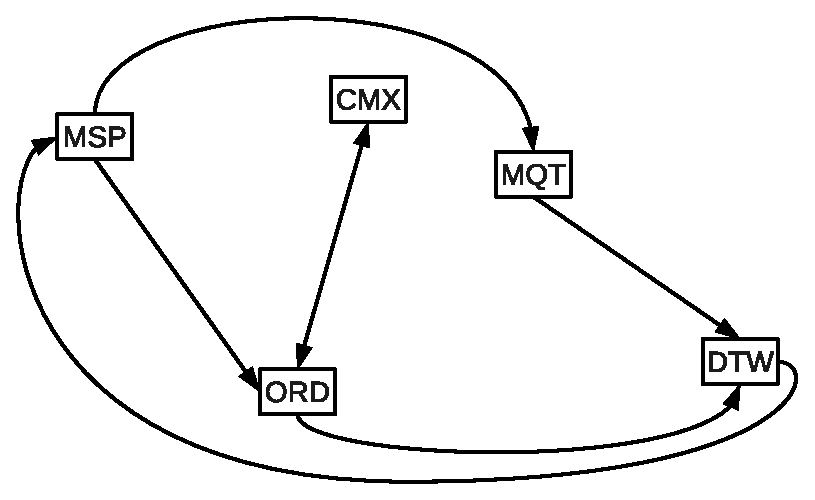
\includegraphics[width=2.2in]{figs/example_relations_fig1}
    % 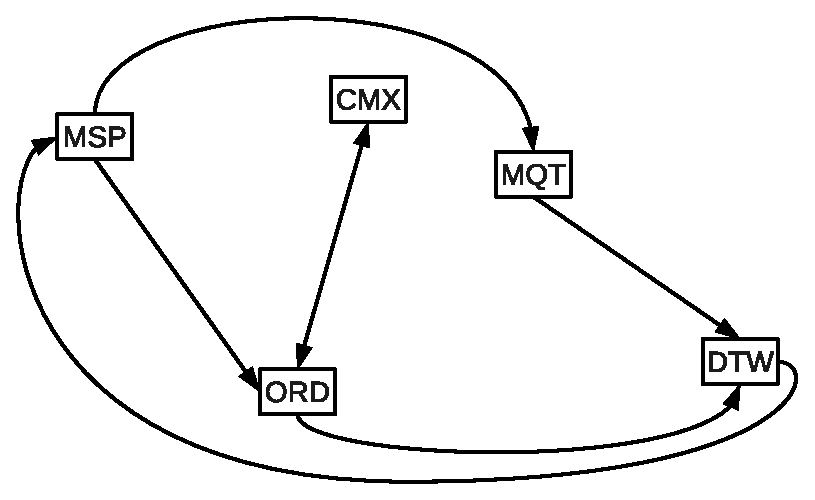
\epsfig{file=figs/example_relations_fig1.eps,width=2.2in}
\end{center}
\else
\begin{center}	
	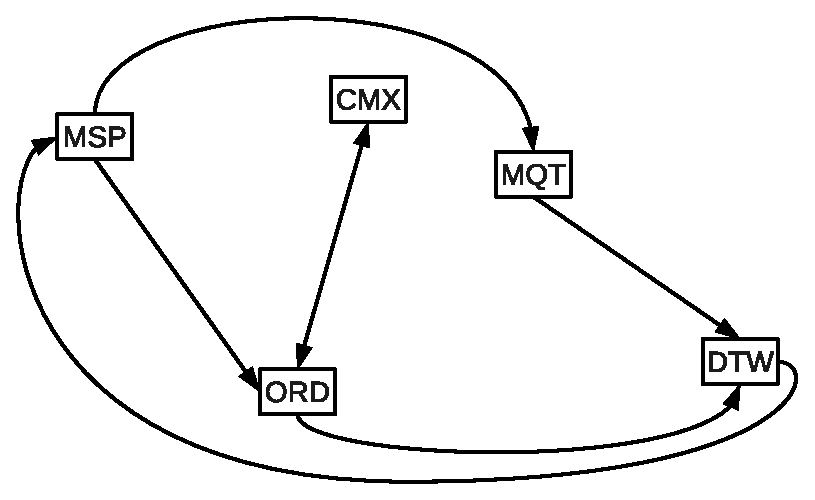
\includegraphics[width=2.2in]{figs/example_relations_fig1}
	% 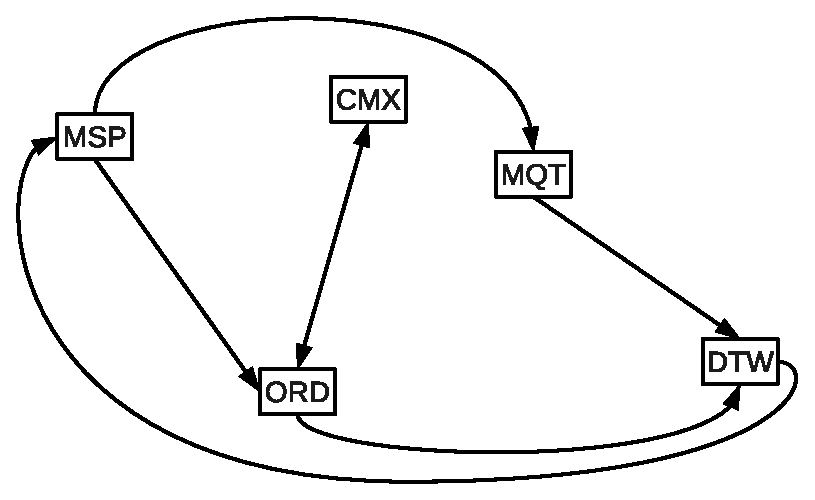
\epsfig{file=figs/example_relations_fig1.eps,width=3.5in}
\end{center}
\fi
\begin{enumerate}[label=(\alph*),itemsep=0pt,parsep=0pt,topsep=0pt,partopsep=0pt]
	\item (1pt) Give the set $A$ the relation $R$ is on.
	\item (1pt) Give the relation $R$ (that is, list the ordered pairs explicitly).
	\item (2pt) Express the relation $R$ as a zero-one matrix (present cities in alphabetic order, e.g., \CMX, \DTW, \MQT, ...)
	\item (2pt) Find the diagonal relation on $A$ (list all ordered pairs explicitly). 
	\item (2pt) Find the reflexive closure of $R$ (list all ordered pairs explicitly).
	\item (2pt) Find $R^{-1}$ (list all ordered pairs explicitly).
	\item (2pt) Find the symmetric closure of $R$. 
	\item (1pt) Describe what the pairs in $R \circ R$ represent.
	\item (2pt) Find $R \circ R$ (list all ordered pairs explicitly). 
	\item (1pt) Describe what the pairs in $R^3$ represent.
	\item (2pt) Find $R^3$ (list all ordered pairs explicitly).
	\item (1pt) Describe what the transitive closure, $R^{*}$ represents.
	\item (3pt) Find $R^{*}$ (list all ordered pairs explicitly).
\end{enumerate}
    \ifprintanswers
        \vspace{-10pt}
    \fi
    \begin{solution}
    \begin{enumerate}[label=(\alph*),itemsep=2pt,parsep=0pt,topsep=0pt,partopsep=0pt]
        \item $\{ \CMX, \DTW, \MQT, \MSP, \ORD \}$
        \item $\{  (\CMX, \ORD), (\DTW, \MSP), (\MQT, \DTW), (\MSP, \MQT), (\MSP, \ORD), \\
        (\ORD, \CMX), (\ORD, \DTW)\}$
        \item $ \mathbf{M}_R = 
            \begin{bmatrix} 
                0 & 0 & 0 & 0 & 1 \\
                0 & 0 & 0 & 1 & 0 \\
                0 & 1 & 0 & 0 & 0 \\
                0 & 0 & 1 & 0 & 1 \\
                1 & 1 & 0 & 0 & 0 \\
            \end{bmatrix} $
        \item $\{  (\CMX, \CMX), (\DTW, \DTW), (\MQT, \MQT), (\MSP, \MSP), (\ORD, \ORD)\}$
        \item $\{  (\CMX, \CMX), (\CMX, \ORD), (\DTW, \DTW), (\DTW, \MSP), (\MQT, \DTW), \\
         (\MQT, \MQT), (\MSP, \MQT), (\MSP, \MSP), (\MSP, \ORD), (\ORD, \CMX), \\
         (\ORD, \DTW), (\ORD, \ORD) \}$
        \item $\{  (\CMX, \ORD), (\DTW, \MQT), (\DTW, \ORD), (\MQT, \MSP), (\MSP, \DTW), \\
        (\ORD, \CMX), (\ORD, \MSP)\}$
        \item $\{  (\CMX, \ORD), (\DTW, \MQT), (\DTW, \MSP), (\DTW, \ORD), (\MQT, \DTW), \\
        (\MQT, \MSP), (\MSP, \DTW), (\MSP, \MQT), (\MSP, \ORD), (\ORD, \CMX), \\
         (\ORD, \DTW), (\ORD, \MSP)\}$
        \item the cities for which you can travel between in two flights
        \item $\{  (\CMX, \CMX), (\CMX, \DTW), (\DTW, \MQT), (\DTW, \ORD), (\MQT, \MSP), \\
        (\MSP, \CMX), (\MSP, \DTW), (\ORD, \MSP), (\ORD, \ORD)\}$ 
        \item the cities for which you can travel between in three flights
        \item $\{  (\CMX, \MSP), (\CMX, \ORD), (\DTW, \CMX), (\DTW, \DTW), (\MQT, \MQT), \\
        (\MQT, \ORD), (\MSP, \MSP), (\MSP, \ORD), (\ORD, \CMX), (\ORD, \DTW), \\
         (\ORD, \MQT), (\ORD, \ORD)  \}$
        \item the cities for which you can travel between in taking $n$ number of flights
        \item $ \{  (\CMX, \CMX), (\CMX, \DTW), (\CMX, \MQT), (\CMX, \MSP), (\CMX, \ORD), \\
        (\DTW, \CMX), (\DTW, \DTW), (\DTW, \MQT), (\DTW, \MSP), (\DTW, \ORD), \\
         (\MQT, \CMX), (\MQT, \DTW), (\MQT, \MQT), (\MQT, \MSP), (\MQT, \ORD), \\
         (\MSP, \CMX), (\MSP, \DTW), (\MSP, \MQT), (\MSP, \MSP), (\MSP, \ORD), \\
         (\ORD, \CMX), (\ORD, \DTW), (\ORD, \MQT), (\ORD, \MSP), (\ORD, \ORD) \}$
    \end{enumerate}
    \end{solution}



% CS2311-f14 hw5
% \gquestion{14}{10}{a-c} Consider the following relations on the sets \textit{Directors} $ = D = \{$\text{Spielberg}, \text{Scorsese}, \text{Bigelow} $\}$, \textit{Movies} $ = M = \{$\text{Saving Private Ryan}, \text{Lincoln}, \text{Catch Me If You Can}, \text{The Departed}, \text{Zero Dark Thirty}, \text{Hurt Locker}  $\}$, \textit{Actors} $= A = \{$\text{Leonardo DiCaprio}, \text{Tom Hanks}, \text{Matt Damon}, \text{Martin Sheen}, \text{Jessica Chastain}, \text{Jeremy Renner} $\}$

% Consider the relation $R$ from \textit{Directors} to \textit{Movies} and $S$ from \textit{Movies} to \textit{Actors}.
% \begin{align*}
% R &= \{ (\text{Spielberg}, \text{Saving Private Ryan}), 
% 		(\text{Spielberg}, \text{Lincoln}), 
% 		(\text{Spielberg}, \text{Catch Me If You Can}), \\
%   		& \quad  (\text{Scorsese}, \text{The Departed}), 
%   		(\text{Bigelow}, \text{Zero Dark Thirty}), 
%   		(\text{Bigelow}, \text{Hurt Locker}) \} \\
% S &= \{ (\text{Saving Private Ryan}, \text{Tom Hanks}), 
% 		(\text{Saving Private Ryan}, \text{Matt Damon}),  \\
%   		& \quad  (\text{Catch Me If You Can}, \text{Leonardo DiCaprio}),
%   		(\text{Catch Me If You Can}, \text{Tom Hanks}), 
%   		(\text{Catch Me If You Can}, \text{Martin Sheen}),  \\
%   		& \quad (\text{The Departed}, \text{Leonardo DiCaprio}), 
%   		(\text{The Departed}, \text{Martin Sheen}),  \\
%   		& \quad (\text{Zero Dark Thirty}, \text{Jessica Chastain}), 
%   		(\text{Hurt Locker}, \text{Jeremy Renner})  \}
% \end{align*}

% This can written in shorthand as: 
% \begin{align*}
%   R &= \{ (Sp, SPR), (Sp, Linc), (Sp, CMIYC), (Sc, Dep), (B, ZDT), (Z, HL) \}
%   S &= \{ (SPR, TH), (SPR, MD), (CMIYC, LD), (CMIYC, TH), (CMIYC, MS), (Dep, LD), (Dep, MS), (ZDT, JC), (HL, JR) \}
% \end{align*}
% 	\ifprintanswers
% 	\else
% 	\begin{enumerate}[label=(\alph*)]
% 		\item What is $S \circ R$ (list the elements in the relation)?
% 		\item Construct $T = S \circ S^{-1}$.
% 		\item What is $T^*$, describe it in words the relation from $X$ to $Y$ with \ldots
% 		\item Calculate $T^*$
% 	\end{enumerate}
% 	\fi

% 	\ifprintanswers
%         \vspace{-30pt}
%     \fi
%     \begin{EnvFullwidth}
%     \begin{solution}
%     \small
%     \begin{enumerate}[label=(\alph*)]
%     	\item What is $S \circ R$? \\
%     	$S \circ R = \{ (Sp, TH), (Sp, MD), (Sp, LD), (Sp, MS), (Sc, LD), (Sc, MS), (B, JC), (B, JR) \}$

%     	% $S \circ R = \{ (\text{Spielberg}, \text{Tom Hanks}), 
%     	% 				(\text{Spielberg}, \text{Matt Damon}), 
%     	% 				(\text{Spielberg}, \text{Leonardo DiCaprio}), \\
%     	% 				(\text{Spielberg}, \text{Martin Sheen}), 
%     	% 				(\text{Scorsese}, \text{Leonardo DiCaprio}), 
%     	% 				(\text{Scorsese}, \text{Martin Sheen}), \\
%     	% 				(\text{Bigelow}, \text{Jessica Chastain}),
%     	% 				(\text{Bigelow}, \text{Jeremy Renner})  \}$
%     	\item $T = S \circ S^{-1}$ \\
%     	$S^{-1} = \{ (TH, SPR), (MD, SPR), (LD, CMIYC), (TH, CMIYC), (MS, CMIYC), (LD, Dep), (MS, Dep), (JC, ZDT), (JR, HL) \}$\\[4pt]
%     	$T = S \circ S^{-1} = \{ (TH, TH), (MD, MD), (LD, LD), (MS, MS), (JC, JC), (JR, JR), \\
%     							(TH, MD), (MD, TH), (TH, LD), (LD, TH), (TH, MS), (MS, TH), (LD, MS), (MS, LD)  \}$
%   		% $T = S \circ S^{-1} = \{  (\text{Tom Hanks}, \text{Tom Hanks}) 
%   		% 			(\text{Matt Damon}, \text{Matt Damon}),  \\
%   		% 			(\text{Leonardo DiCaprio}, \text{Leonardo DiCaprio}), 
%   		% 			(\text{Martin Sheen}, \text{Martin Sheen}), \\
%   		% 			(\text{Jessica Chastain}, \text{Jessica Chastain}), 
%   		% 			(\text{Jeremy Renner}, \text{Jeremy Renner}), \\
%   		% 			(\text{Tom Hanks}, \text{Matt Damon}), 
%   		% 			(\text{Matt Damon}, \text{Tom Hanks}), \\
%   		% 			(\text{Leonardo DiCaprio}, \text{Martin Sheen}), 
%   		% 			(\text{Martin Sheen}, \text{Leonardo DiCaprio})  \}$
%   		\item $T$ is the relation from \textit{Actors} to \textit{Actors} with the first actor appearing in a film with the second.
%   		\item  $T^* = \{  (TH, TH), (MD, MD), (LD, LD), (MS, MS), (JC, JC), (JR, JR), \\
%     							(TH, MD), (MD, TH), (TH, LD), (LD, TH), (TH, MS), (MS, TH), (LD, MS), (MS, LD) \}$
%     \end{enumerate}
%     \end{solution}
%     \end{EnvFullwidth}


	\ifprintanswers
        \vspace{-5pt}
    \fi
\gquestion{11}{6}{a-b,d(i)-(iii)} Let the sets \textit{Director}, $D$, be a set of movie directors, \textit{Movie}, $M$, be a set of movies, and \textit{Actor}, $A$, be a set of actors.  We define the following relations: 
\begin{itemize}
	\item $appearedIn \s $ \textit{Actor} $\times$ \textit{Movie} or $appearedIn \s A \times M$, where \\  $a \;appearedIn\; m$ if $a$ was an actor who appeared in movie $m$
	\item $directedFilm \s $\textit{Director} $\times$ \textit{Movie} or $directedFilm \s D \times M$, where \\
	$d \;directedFilm\; m$ if $d$ was the director of movie $m$ 
	\item $starredIn \s $\textit{Actor} $\times$ \textit{Movie} of $starredIn \s A \times M$, where \\
	$a \;starredIn\; m$ if $a$ was an actor with top 3 billing in movie $m$ 
\end{itemize}

Express the following using only set operations and relations: 
\begin{enumerate}[label=(\alph*),itemsep=2pt,parsep=0pt,topsep=0pt,partopsep=0pt]
	\item There must be actors who have both appeared in and starred in a movie. 
	\item Some people appear in movies they direct. 
	\item Some movies are directed by people who do not star in them. 
\end{enumerate}

Take the following relations and express what they mean in English.  Think about what sets define the elements the relations is made up of. 
\begin{enumerate}[label=(\alph*),itemsep=2pt,parsep=0pt,topsep=0pt,partopsep=0pt]
	\setcounter{enumi}{3}
	\item $appearedIn \circ appearedIn^{-1}$ \\
	Is this relation (i) reflexive? (ii) symmetric? and (iii) transitive?
	% \begin{enumerate}[label=(\roman*),itemsep=2pt,parsep=0pt,topsep=0pt,partopsep=0pt]
	% 	\item is the relation reflixive?
	% 	\item is the relation symmetric? 
	% 	\item is the relation transitive? 
	% \end{enumerate}
	\item $directedFilm \circ starredIn^{-1}$ \\
	Is this relation (i) reflexive? (ii) symmetric? and (iii) transitive?
	% \begin{enumerate}[label=(\roman*),itemsep=2pt,parsep=0pt,topsep=0pt,partopsep=0pt]
	% 	\item is the relation reflixive?
	% 	\item is the relation symmetric? 
	% 	\item is the relation transitive? 
	% \end{enumerate}
\end{enumerate}	
    \ifprintanswers
        \vspace{-10pt}
    \fi
    \begin{solution}
    \begin{enumerate}[label=(\alph*),itemsep=2pt,parsep=0pt,topsep=0pt,partopsep=0pt]
    	\item $appearedIn \cap starredIn \neq \es $
    	\item $directedFilm \cap appearIn \neq \es$ 
    	\item $directedFilm \not\s starredIn $ 
  %   	\item This relation could be termed \textit{appearsWith} it is defined as $\s A \times A$, where $(x,y)$ in the relation if actor $x$ appeared with actor $y$ in a movie. 
		% \begin{enumerate}[label=(\roman*),itemsep=2pt,parsep=0pt,topsep=0pt,partopsep=0pt]
		% 	\item Yes 
		% 	\item Yes 
		% 	\item 
		% \end{enumerate}
        \item This relation is defined as $\s M \times M$, where $(x,y)$ in the relation if movie $x$ shared actors with movie $y$.  Many of this properties can be seen with the following example. 
            \begin{quote}
                (HarrisonFord, Star Wars), (HarrisonFord, Blade Runner 2049), (Robin Wright, Blade Runner 2049), (Robin Wright, The Princess Bride) $\in appearedIn$ 
            \end{quote}
        So, $appearedIn \circ appearedIn^{-1}$ would have the following elements: 
        
        \scriptsize
        \begin{center}
        \begin{tabular}{rll}
          $(m, a) \in appearedIn^{-1}$  & $ (a, m) \in appearedIn$  & $appearedIn \circ appearedIn^{-1}$ \\
          \hline 
            (Star Wars, HarrisonFord) & (HarrisonFord, Blade Runner 2049) & 
                (Star Wars, Blade Runner 2049) \\
            (Blade Runner 2049, HarrisonFord) & (HarrisonFord, Blade Runner 2049) & 
                (Blade Runner 2049,  Blade Runner 2049) \\
            (Blade Runner 2049, Robin Wright) & (Robin Wright, The Princess Bride) & 
                (Blade Runner 2049, The Princess Bride) \\
            \ldots & & 
        \end{tabular}
        \end{center}
        \normalsize

            \begin{enumerate}[label=(\roman*),itemsep=2pt,parsep=0pt,topsep=0pt,partopsep=0pt]
              \item Yes, every movie shares an actor with itself 
              \item Yes, if movie a shares an actor with movie b, movie b will also share an actor with a
              \item No, e.g, Star Wars and Blade Runner are connected via Harrison Ford and Blade Runner and The Princess Bride are connected via Robin Wright, but that doesn't mean Star Wars and The Princess Bride are paired.
            \end{enumerate}


		\item This relation is defined as $\s M \times M$, where $(x,y)$ in relation if $x$ was directed by the actor who starred in $y$.  Note, this assumes there is an overlap between actors and directors which there is in practice.
		\begin{enumerate}[label=(\roman*),itemsep=2pt,parsep=0pt,topsep=0pt,partopsep=0pt]
			\item No 
            % actors can star in a movie they don't direct
			\item No 
            % actors can star in a movie they don't direct or direct a movie they do not star in
			\item No
		\end{enumerate}
    \end{enumerate}
    \end{solution}



% \ugquestion{2} Rosen Ch 9.4 \# 4, p. 606
%     \ifprintanswers
%         \vspace{-10pt}
%     \fi
%     \begin{solution}
%     How can the directed graph representing the reflexive closure of a
%     relation on a finite set be constructed from the directed graph of
%     the relation?
%     \begin{quote}
%         Start with the original graph for the relationa and add any missing self-loops, $a \ra a$ for every node.
%     \end{quote}
%     \end{solution}


% \ugquestion{2} Rosen Ch 9.4 \#8, p. 606
% 	\ifprintanswers
%         \vspace{-10pt}
%     \fi
%     \begin{solution}
%     How can the directed graph representing the symmetric closure of a relation on a finite set be constructed from the directed graph of the relation?
%     \begin{quote}
%         Start with the original graph for the relation and for each edge $a \ra b$, add the edge $b \ra a$ if it is not already there.
%     \end{quote}
%     \end{solution}



	\ifprintanswers
        \vspace{-5pt}
    \fi
% Equivalence Relations
\gquestion{8}{2}{e} Rosen Ch 9.5.2(a,c-e) p. 646
    \ifprintanswers
        \vspace{-15pt}
    \fi
    \begin{EnvFullwidth}
    \begin{solution}
    Which of these relations on the set of all people are equivalence relations?  Determine the properties of an equivalence relation that the others lack. 
        % \begin{tabular}{l}
    \begin{itemize}[itemsep=2pt,parsep=0pt,topsep=0pt,partopsep=0pt]
        \item[] (a) $\{(a,b) \;|\; a \;\text{and}\; b \;\text{are the same age}\;\}$.
          Equivalence relation 
%        a) $\{(a,b) \;|\; a \;\text{and}\; b \;\text{are the same age}\;\}$. \\
        % b) $\{(a,b) \;|\; a \;\text{and}\; b \;\text{have the same parents}\;\}$. \\
        % Equivalence relation\\
        
       \item[] (c) $\{(a,b) \;|\; a \;\text{and}\; b \;\text{share a common parent}\;\}$.  
       Not an equivalence relation, not transitive
       \item[] (d) $\{(a,b) \;|\; a \;\text{and}\; b \;\text{have met}\;\}$.         
       No, It is not transitive.
       \item[] (e) $\{(a,b) \;|\; a \;\text{and}\; b \;\text{speak a common language}\;\}$. 
       Not an equivalence relation, not transitive 
    \end{itemize}
        % \end{tabular}
    \end{solution}
    \end{EnvFullwidth}




    \ifprintanswers
        \vspace{-5pt}
    \fi
\ugquestion{4}  Let $R_m$ be the relation on $\Zp$ where $R_m = \{ (a,b) \;|\; a \equiv b\; ({mod}\; m )\}$.
\begin{enumerate}[label=(\alph*),itemsep=1pt,topsep=1pt]
	\item Give the four members of $[ 4 ]_{R_2}$ with the smallest values.
	\item Give the four members of $[ 4 ]_{R_6}$ with the smallest values.
	\item Give the four members of $[ 5 ]_{R_3}$ with the smallest values.
	\item How many unique equivalence classes for $R_7$ exist on the members of $\Zp$.
\end{enumerate}
    \ifprintanswers
        \vspace{-12pt}
    \fi
    \begin{solution}
    \begin{enumerate}[label=(\alph*),itemsep=1pt,topsep=0pt]
    	\item $[ 4 ]_{R_2} = \{ 2, 4, 6, 8 ,\ldots \}$
    	\item $[ 4 ]_{R_6} = \{ 4, 10, 16, 22, \ldots \}$
    	\item $[ 5 ]_{R_3} = \{ 2, 5, 8, 11, \ldots \}$
        % {0, 3, 6, 9, 12 } or {1, 4, 7, 10, 13 } or 
        %  { 2, 5, 8, 11, 14}

    	\item There are 7 unique equivalence classes for $R_7$ 
    \end{enumerate}
    \end{solution}



	\ifprintanswers
        \vspace{-10pt}
    \fi
\gquestion{3}{2}{(a,b)} Rosen Ch 9.5.24, p. 647.  \\
If it is an equivalence relation, list the equivalence classes assuming the elements are ordered $x_1, x_2, x_3, x_4, \dots$. 
	\ifprintanswers
        \vspace{-15pt}
    \fi
    \begin{solution}
    	\begin{enumerate}[label=(\alph*),itemsep=1pt,topsep=0pt]
    		\item The relation is not symmetric, therefore, it is not an equivalence relation. 
    		\item The relation is an equivalence relation. \\
    		The equivalence classes are $\{x_1, x_3\}, \{x_2, x_4\}$
    		\item The relation is an equivalence relation. \\
    		The equivalence classes are $\{ x_1, x_2, x_3 \}, \{ x_4 \}$
    	\end{enumerate}
    \end{solution}



    \ifprintanswers
        \vspace{-10pt}
    \fi
\ugquestion{3} Rosen Ch 9.5.56(a,b), p.649
    \ifprintanswers
        \vspace{-15pt}
    \fi
    \begin{solution}
    	\begin{enumerate}[label=(\alph*),itemsep=1pt,topsep=0pt]
    		\item \textbf{No, not necessarily}. \\
    		Let $R_1$ and $R_2$ be defined over $\{0,1,2\}$. $R_1$ has equivalence classes $\{0\}$ and $\{1,2\}$; $R_2$ has equivalence classes $\{0,2\}$ and $\{1\}$. Then $R_1 \cup R_2$ is not transitive, since $(0, 2) \in R_2$ (and therefore $R_1 \cup R_2$ ) and $(2, 1) \in  R_1$ (and therefore $R_1 \cup R_2$), but $(0, 1) \not\in R_1 \cup R_2$.

    		\item \textbf{Yes} $R_1 \cap R_2$ must be an equivalence relation. \\
    		If $R_1$ and $R_2$ are reflexive, then the intersection must also then be reflexive. 

		    If $R_1$ and $R_2$ are both symmetric, then the intersection of $R$ and $R_2$ must also be symmetric.

		    If $R_1$ and $R_2$ are both transitive, then the intersection of $R_1$ and $R_2$ is also transitive.

    	\end{enumerate}
    \end{solution}


    \ifprintanswers
        \vspace{-10pt}
    \fi
\gquestion{2}{2}{all} Rosen Ch 9.6.4(a,c), p. 662.
    \ifprintanswers
        \vspace{-15pt}
    \fi
    \begin{solution}
    \begin{itemize}[itemsep=0pt,parsep=0pt,topsep=0pt,partopsep=0pt]
        \item[(a)] There should be unequal people of the same height, therefore, the relation is not antisymmetric and $(S, R)$ is not a poset.
        \item[(c)] This is a poset, R is reflexive, antisymmetric, and transitive.
    \end{itemize}
    \end{solution}





    \ifprintanswers
        \vspace{-10pt}
    \fi
\gquestion{6}{3}{c-f} Which of the following are posets? 
\ifprintanswers
        \vspace{-15pt}
\else
\begin{enumerate}[label=(\alph*),itemsep=0pt,parsep=0pt,
topsep=0pt,partopsep=0pt]
	\item $(\Z, =)$
	\item $(\Z, \neq)$
	\item $(\Z, \geq)$
	\item $(\R, =)$
	\item $(\R, <)$
	\item $(\R, \geq)$
\end{enumerate}
\fi
    \begin{solution}
    \begin{enumerate}[label=(\alph*),itemsep=0pt,parsep=0pt,
		topsep=0pt,partopsep=0pt]
		\item $(\Z, =)$, Yes
		\item $(\Z, \neq)$, No, it is not reflexive. 
		\item $(\Z, \geq)$, Yes
		\item $(\R, =)$, Yes
		\item $(\R, <)$, No, it is not reflexive.
		\item $(\R, \geq)$, Yes
	\end{enumerate}
    \end{solution}



    \ifprintanswers
        \vspace{-10pt}
    \fi
\ugquestion{6} Rosen Ch 9.6.32(a-f), p. 663.
    \ifprintanswers
        \vspace{-15pt}
    \fi
    \begin{solution}
    \begin{enumerate}[label=(\alph*),itemsep=0pt,parsep=0pt,topsep=0pt,partopsep=0pt]
        \item maximal elements: $\{ l, m\}$
        \item minimal elements: $\{ a, b, c \}$
        \item there is no greatest element
        \item there is no least element
        \item $\{ k, l, m\}$
        \item $\{ k \}$
    \end{enumerate}
    \end{solution}


    \ifprintanswers
        \vspace{-10pt}
    \fi
\section*{Graphs}


\ugquestion{9}\label{p1} Use a graph to model the following problems: 
\begin{parts}
	\part Twitter ``follows" - 
	Construct a graph of who follows who on Twitter on a set of people.  \\
	Ann follows Bob, Ann also follows Charlie, Bob follows Ann, Bob also follows Ed, Charlie follows Dana, Dana follows Bob, Dana also follows Flora, Ed follows Ann, Ed also follows Charlie. 

	\part Integer division -Construct a graph that models whether for a pair of integers, one integer even divides the other. \\ Consider the set of integers $V = \{2, 3, 4, 6, 8, 9, 12, 18, 27 \}$; two vertices are adjacent if one evenly divides the other. 

	\part Airline flights \\
	An airline has the following direct flights on their system, where each direct route between city $a$ and $b$ \underline{and back} is listed below.  Model the all the routes on the system as a graph.  
	\begin{tabular}{ccc|ccc}
		City $a$ & City $b$ & \# of flights & City $a$ & City $b$ & \# of flights \\
		\hline
			Atlanta & Chicago & 1 			& Chicago & San Francisco & 2 \\
			Atlanta & Miami & 1 			& Denver & Los Angeles & 2 \\
			Atlanta & New York & 1 			& Denver & San Francisco & 1 \\
			Boston & New York & 2 			& Los Angeles & New York & 3 \\
			Boston & Chicago & 1 			& Los Angeles & San Francisco & 2 \\
			Chicago & Denver & 1 			& Miami & New York & 1 \\
			Chicago & New York & 2 			&  New York & San Francisco & 2 \\
		\hline
	\end{tabular}

\end{parts}
	\ifprintanswers
		\vspace{-10pt}
	\fi
	\begin{EnvFullwidth}
	\begin{solution}
		\begin{tabular}{ccc}
        (a) follows graph 
        & (b) integer division graph 
        & (c) airline flights graph \\
\begin{tikzpicture}[scale=0.5]
    %\GraphInit[vstyle=Welsh]
    \tikzset{VertexStyle/.style = {shape = circle,
                                    %ball color = orange,
                                    text = black,

                                    inner sep = 1pt,
                                    % outer sep = 0pt,
                                    minimum size = 14 pt,
                                    draw=black}}
    \tikzset{edge/.style = {->, black,line width=1pt}}
    \SetGraphUnit{3}
    \Vertex[x=0,y=3]{A}
    \Vertex[x=3,y=3]{B}
    \Vertex[x=6,y=3]{C}
    \Vertex[x=6,y=0]{D}
    \Vertex[x=3,y=0]{E}
    \Vertex[x=0,y=0]{F}
    % \Vertex[x=0,y=0,Lpos=180,LabelOut]{Gr}
    % \AddVertexColor{blue!50}{Gr}
    % \Vertex[x=4,y=0,Lpos=0,LabelOut]{CM}
    % \AddVertexColor{blue}{CM}
    % \Vertex[x=0,y=4,Lpos=180,LabelOut]{Er}
    % \AddVertexColor{orange!60}{Er}
    % \Vertex[x=4,y=4,Lpos=0,LabelOut]{Be}
    % \AddVertexColor{orange!40}{Be}
    % \Vertex[x=2,y=5.5,Lpos=0,LabelOut]{Co}
    % \AddVertexColor{purple!80}{Co}
    % \Vertex[x=2,y=4,Lpos=0,LabelOut]{Os}
    % \AddVertexColor{green!80}{Os}
    % \Vertex[x=2,y=2,Lpos=0,LabelOut]{BB}
    % \AddVertexColor{yellow}{BB}
    \tikzset{EdgeStyle/.style = {->,line width=1pt}}
    \Edge(B)(E)
    \Edge(C)(D)
    \Edge(D)(B)
    \Edge(E)(C)
    % \Edge(E)(A)
    \draw[edge] (A) to [->,out=60,in=120] (C);
    \draw[edge] (E) to [->,out=135,in=-90] (A);
    \tikzset{EdgeStyle/.style = {black,->,line width=1pt,bend left}}
    \Edge(A)(B)
    % \Edge(A)(C)
    \Edge(B)(A)
    \Edge(D)(F)
    % \Edge(Gr)(CM)
    % \Edge(Gr)(BB)
    % \Edge(Er)(Gr)
    % \Edge(Er)(BB)
    % \Edge(Be)(CM)
    % \Edge(Be)(BB)
    % \Edge(Co)(Er)
    % \Edge(Co)(Be)
    % \Edge(Os)(Co)
    % \Edge(BB)(Os)
\end{tikzpicture}

&

\hspace*{0.2in}
\begin{tikzpicture}[scale=0.5]
    %\GraphInit[vstyle=Welsh]
    \tikzset{VertexStyle/.style = {shape = circle,
                                    %ball color = orange,
                                    text = black,
                                    inner sep = 1pt,
                                    outer sep = 0pt,
                                    minimum size = 4 pt,
                                    draw=black}}
    \SetGraphUnit{2}
    \Vertex[x=0,y=0,Lpos=-90,LabelOut]{8}
    \Vertex[x=0,y=4,Lpos=90,LabelOut]{4}
    \Vertex[x=4,y=0,Lpos=-70,LabelOut]{18}
    \Vertex[x=4,y=4,Lpos=120,LabelOut]{12}
    \Vertex[x=2,y=2,Lpos=-90,LabelOut]{2}
    \Vertex[x=4,y=2,Lpos=-45,LabelOut]{6}
    \Vertex[x=6,y=2,Lpos=-90,LabelOut]{3}
    \Vertex[x=8,y=0,Lpos=-90,LabelOut]{9}
    \Vertex[x=8,y=4,Lpos=90,LabelOut]{27}
    \tikzset{EdgeStyle/.style = {black,line width=1pt}}
    \Edge(8)(4)
    \Edge(8)(2)
    \Edge(4)(2)
    \Edge(4)(12)
    \Edge(2)(18)
    \Edge(2)(6)
    \Edge(2)(12)
    \Edge(18)(6)
    \Edge(18)(3)
    \Edge(18)(9)
    \Edge(6)(12)
    \Edge(6)(3)
    \Edge(12)(3)
    \Edge(3)(9)
    \Edge(9)(27)
    \Edge(3)(27)
    % \tikzset{EdgeStyle/.style = {loop}}
    % \Edge(2)(2)
    % \Edge(3)(3)
    % \Edge(4)(4)
    % \Edge(6)(6)
    % \Edge(8)(8)
    % \Edge(9)(9)
    % \Edge(12)(12)
    % \Edge(18)(18)
    % \Edge(27)(27)
    \tikzset{edge/.style = {black,line width=1pt}}
    \draw[edge] (2) to [in=145,out=215,distance=30pt] (2);
    \draw[edge] (3) to [in=35,out=-35,distance=30pt] (3);
    \draw[edge] (4) to [in=135,out=225,distance=30pt] (4);
    \draw[edge] (6) to [in=10,out=80,distance=30pt] (6);
    \draw[edge] (8) to [in=135,out=225,distance=30pt] (8);
    \draw[edge] (9) to [in=45,out=-45,distance=30pt] (9);
    \draw[edge] (12) to [in=65,out=-25,distance=30pt] (12);
    \draw[edge] (18) to [in=155,out=245,distance=30pt] (18);
    \draw[edge] (27) to [in=45,out=-45,distance=30pt] (27); 
\end{tikzpicture}

&
% \multicolumn{2}{c}{
\begin{tikzpicture}[scale=0.85]
    %\GraphInit[vstyle=Welsh]
    \tikzset{VertexStyle/.style = {shape = circle,
                                    %ball color = orange,
                                    color=black,
                                    text = black,
                                    inner sep = 1pt,
                                    outer sep = 0pt,
                                    minimum size = 4 pt,
                                    draw}}
    \SetGraphUnit{2}
    \Vertex[x=0,y=0,Lpos=180,LabelOut]{LA}
    \Vertex[x=2,y=1.2,Lpos=90,LabelOut]{Den}
    \Vertex[x=4,y=1.8,Lpos=90,LabelOut]{Chi}
    \Vertex[x=5.2,y=2,Lpos=0,LabelOut]{NY}
    \Vertex[x=4.3,y=0.2,Lpos=-90,LabelOut]{Atl}
    \Vertex[x=5.7,y=2.8,Lpos=0,LabelOut]{Bos}
    \Vertex[x=4.8,y=-1,Lpos=-90,LabelOut]{Mia}
    \Vertex[x=-0.3,y=1.3,Lpos=180,LabelOut]{SF}
    \tikzset{EdgeStyle/.style = {black,line width=0.75pt}}
    \Edge(Atl)(Chi)
    \Edge(Atl)(Mia)
    \Edge(Atl)(NY)
    \Edge(Bos)(Chi)
    \Edge(Chi)(Den)
    \Edge(Den)(SF)
    \Edge(Mia)(NY)
    \tikzset{EdgeStyle/.style = {black,line width=0.75pt,bend left}}
    \Edge(Bos)(NY)
    \Edge(Chi)(NY)
    % \Edge(Chi)(SF)
    % \Edge(Den)(LA)
    % \Edge(Chi)(SF)
    \Edge(LA)(SF)
    % \Edge(NY)(SF)
    \tikzset{EdgeStyle/.style = {black,line width=0.75pt,bend right}}
    \Edge(Bos)(NY)
    \Edge(Chi)(NY)
    \Edge(Chi)(SF)
    % \Edge(Den)(LA)
    \Edge(LA)(SF)
    \tikzset{EdgeStyle/.style = {black,line width=0.75pt}}
    \draw[EdgeStyle] (Chi) to [out=130,in=60] (SF);
    \draw[EdgeStyle] (LA) to [out=15,in=-135] (Den);
    \draw[EdgeStyle] (LA) to [out=50,in=-160] (Den); 
    \draw[EdgeStyle] (LA) to [out=10,in=-145] (NY);
    \draw[EdgeStyle] (LA) to [out=0,in=-135] (NY);
    \draw[EdgeStyle] (LA) to [out=-15,in=-125] (NY);
    \draw[EdgeStyle] (SF) to [out=110,in=110] (NY);
    \draw[EdgeStyle] (SF) to [out=80,in=130] (NY);
    
    % \draw(NY) to [out=120,in=90] (SD);
    % \draw(Chi) to [out=280,in=-25] (SD);

\end{tikzpicture}
% }
\end{tabular}
\vspace{-5pt} 
	\end{solution}
	\end{EnvFullwidth}



\gquestion{3}{2}{a-b} Determine the type of graphs depicted in each part of Problem \ref{p1}: simple graph? multigraph? pseudograph? directed graph? directed multigraph?
	\ifprintanswers
		\vspace{-10pt}
	\fi
	\begin{solution}
		(a) directed graph  \\[2pt]
		(b) pseudograph   \\[2pt]
		(c) multigraph
	\end{solution}

	\ifprintanswers
		\vspace{-10pt}
	\fi

\gquestion{3}{3}{all} For the graphs in Problem \ref{p1}(a-c), determine the number of vertices and edges.
	\ifprintanswers
		\vspace{-10pt}
	\fi
	\begin{solution}
		(a) $|V| = 6$, $|E| = 9$

		(b) $|V| = 9$, $|E| = 25$ %(without loops $|V| = 8$, $|E| = 16$) \\

		(c) $|V| = 8$, $|E| = 22$
	\end{solution}




\gquestion{6}{2}{a}  For the graphs in Problem \ref{p1}(a-c), determine degree of each vertex (for directed graphs, indicate both the in-degree and out-degree of each vertex).
	\ifprintanswers
		\vspace{-10pt}
	\fi
	\begin{solution}
		(a) \begin{tabular}{r|cccccc|}
				 & A & B & C & D & E & F  \\
				\hline
				in-degree &  2 & 2 & 2 & 1 & 1 & 1  \\
				out-degree & 2 & 2 & 1 & 2 & 2 & 0   \\
			\end{tabular}

		(b) deg(2)=7, deg(3)=7, deg(4)=5, deg(6)=6, deg(8)=4, deg(9)=5, deg(12)=6, deg(18)=6, deg(27)=4 \\[3pt]
		(c) deg(Atl) = 3, deg(Bos) = 3, deg(Chi) = 7, deg(Den) = 4, deg(Mia) = 2, deg(LA) = 7, deg(NY) = 11, deg(SF) = 7
	\end{solution}



\ugquestion{6} Draw these graphs. \textbf{(a)} $C_5 \quad \quad$ \textbf{(b)} $W_7 \quad \quad$ \textbf{(c)} $K_{3,4}$
	\ifprintanswers
	    \vspace{-10pt}
	\fi
	\begin{solution}
		\begin{tabular}{ccc}

(a)
\begin{tikzpicture}[scale=0.3]
	\SetGraphUnit{2}
	\GraphInit[vstyle=Simple]
	\tikzset{VertexStyle/.style = {
							shape = circle,
							fill = black,
							inner sep = 0pt,
							outer sep = 0pt,
							minimum size = 3pt,
							draw}}
	% \SetVertexSimple[Shape=circle, MinSize=3pt, FillColor=black]
    % \SetUpVertex[NoLabel]
	\grCycle[RA=3]{5}
\end{tikzpicture}

& 
(b)
\begin{tikzpicture}[scale=0.3]
	\SetGraphUnit{3}
	\GraphInit[vstyle=Simple]
	\tikzset{VertexStyle/.style = {
						shape = circle,
						fill = black,
						inner sep = 0pt,
						outer sep = 0pt,
						minimum size = 3pt,
						draw}}
	\grWheel[RA=3]{8}
\end{tikzpicture}

& 
(c)
\begin{tikzpicture}[scale=0.4]
	\SetGraphUnit{3}
	\GraphInit[vstyle=Simple]
	\tikzset{VertexStyle/.style = {
						shape = circle,
						fill = black,
						inner sep = 0pt,
						outer sep = 0pt,
						minimum size = 3pt,
						draw}}
	\grCompleteBipartite[RA=2,RB=2,RS=3]{3}{4}
\end{tikzpicture}


\end{tabular}
	\end{solution}



\gquestion{6}{4}{a-b} For which values of $n$ are (a) $C_n$, (b) $K_n$ and (c) $W_n$ bipartite? Explain your answer.
	\ifprintanswers
	    \vspace{-10pt}
	\fi
	\begin{solution}
		(a) $C_n$:  if $n$ is even, the cycle graph is bipartite, if $n$ is odd, the graph is not bipartite \\[2pt]
		(b) $K_n$:  for $n=2$, the complete graph is bipartite, for $n\geq3$, the graphs are not bipartite (contain triangles)\\[2pt]
		(c) $W_n$: there are no values of $n$ where the wheel graph is bipartite; every graph contains triangle.
	\end{solution}





\gquestion{4}{4}{all} \begin{parts} \part A simple graph with $|V| = n$ and $|E| = 17$ has one vertex of degree 1, two vertices of degree 2, one vertex of degree 3, and two vertices of degree 5. The remaining vertices of the graph have degree 4. What is n?
\part A graph with $|V| = 25$ and $|E| = 62$ has vertices of degree 3, 4, 5, or 6. There are two vertices of degree 4 and 11 vertices of degree 6. How many vertices of the graph have degree 3?
\end{parts}
	\ifprintanswers
	    \vspace{-12pt}
	\fi
	\begin{solution} Use the handshaking theorem:
	\begin{parts}
		\part $1+2+1+x+2=n$ Sum of vertices = n \\
		 $1\cdot 1 + 2\cdot 2 + 1\cdot 3 + x\cdot 4 + 2\cdot 5 = 2\cdot 17$ Handshaking theorem, \\
		 $\rightarrow x = 4$, $\therefore \mathbf{n = 10}$ 
		\part $x+2+y+11=25$ Sum of \# of vertices, where $x$ is \# with degree 3 \\
		$3\cdot x + 4\cdot 2 + 5\cdot y + 6\cdot 11 = 2\cdot 62$ Handshaking theorem, \\
		2 equations, 2 unknowns, solve for x, $\mathbf{x = 5}$
	\end{parts}
	\end{solution}

\section*{Bonus}


\bonusquestion[2] List all the equivalence relations on the set $\{a, b, c\}$.  (Describe the relation be describing the partition on the set).
    \ifprintanswers
        \vspace{-10pt}
    \fi
    \begin{solution}
    There are five such relations
    \[ \{ \{a\}, \{b\}, \{c\} \}; \{ \{a, b\}, \{c\} \}; \{ \{a, c\}, \{b\} \}; 
        \{ \{b, c\}, \{a\} \};  \{ \{a, b, c\} \} \]
    \end{solution}

\end{questions}

\end{document}
